\section{问题重述与建模目标}

题目给出由 Tensor 和 Op 构成的计算图。Tensor 表示算子之间传递的数据，Op 表示需要在处理器流水线上执行的计算操作；边表示数据依赖。问题一要求将普通 Op 划分成若干子图，每个子图作为一个独立 Task 分配到一个核心，并给出每个核心上的 Task 执行顺序。官方评估器在给定方案上模拟核内流水线、片上存储和 DDR 传输，最后以所有操作完成时刻的最大值作为 Makespan。

本文采用如下优化口径：
\begin{enumerate}
  \item 目标函数使用官方问题一评估器返回的 Makespan，而不是将近似评分直接当作最终成绩；
  \item 对每个用例保留单核基准 $M_1$，以 $S_5=M_1/M_5$ 计算 5 核加速比；
  \item 只接受官方 Makespan 严格下降的候选方案，未改善方案沿用已有合法方案；
  \item 所有普通 Op 必须恰好被覆盖一次，原始 \texttt{COPY\_IN}/\texttt{COPY\_OUT} 不写入子图映射，由评估器按照题目规则补充。
\end{enumerate}

\section{图模型、符号与约束}

\subsection{Tensor--Op 图与 Op-DAG}

记原始计算图为 $G=(V,E)$，其中 $V=O\cup T$，$O$ 为 Op 集合，$T$ 为 Tensor 集合。去除原始复制节点后得到普通 Op 集合 $O'\subseteq O$。对于 Tensor $t$，记生产者为 $p(t)$，消费者集合为 $C(t)$；若 $u\in O'$ 生产 $t$ 且 $v\in C(t)$，则在收缩图中加入边 $(u,v)$，得到
\begin{equation}
G_{\mathrm{op}}=(O',E_{\mathrm{op}}),\qquad
(u,v)\in E_{\mathrm{op}}\Longleftrightarrow
\exists t\in T:\ u\to t\to v .
\end{equation}

在 Op-DAG 上使用 Kahn 算法获得拓扑序。拓扑序只用于生成候选和构造核内顺序；候选方案生成后，还要在子图收缩图上再次检查无环，因为原图无环并不能保证任意切分后的 Task 图无环。

\subsection{决策变量}

设候选子图集合为 $\mathcal G=\{1,\ldots,G\}$，核心集合为 $\mathcal K=\{1,\ldots,K\}$。定义
\begin{equation}
x_{u,g}=\begin{cases}1,&u\text{ 属于子图 }g,\\0,&\text{否则},\end{cases}
\qquad
y_{g,k}=\begin{cases}1,&g\text{ 分配到核心 }k,\\0,&\text{否则}.
\end{cases}
\end{equation}
对核心 $k$ 上的子图顺序记为 $\pi_k=(g_{k,1},g_{k,2},\ldots)$。核心编号、子图编号和顺序均由方案 JSON 中的 `node\_to\_subgraph` 与 `core\_schedules` 唯一确定。

\subsection{可行性约束}

普通 Op 的覆盖约束为
\begin{equation}
\sum_{g=1}^{G}x_{u,g}=1,\qquad \forall u\in O'.
\end{equation}
每个子图只能分配到一个核心，每个子图也只能在一个核心顺序中出现一次：
\begin{equation}
\sum_{k=1}^{K}y_{g,k}=1,\qquad
g\in\bigcup_{k=1}^{K}\pi_k .
\end{equation}
令 $H_{\mathcal G}$ 为将同一子图内的 Op 收缩后的 Task 依赖图，则必须满足
\begin{equation}
H_{\mathcal G}\text{ 无环},
\qquad
g\prec_{\pi_k}h\ \text{时不能违反 }g\to h\text{ 的依赖关系}.
\end{equation}
此外，$y_{g,k}$ 的核心下标必须落在 $1,\ldots,K$，每个子图必须覆盖原图中的普通 Op，方案结构还必须通过官方 `validate\_multicore\_plan` 检查。

\section{问题一的精确评价与代理目标}

\subsection{官方 Makespan 目标}

问题一中，子图之间的数据依赖通过 DDR 传递，同核相邻 Task 之间有固定等待，跨核依赖有更大的等待。给定完整方案 $\mathcal S=(x,y,\pi)$ 后，官方事件模拟器隐式计算所有流水线和存储事件，记其输出为
\begin{equation}
M_1(\mathcal S)=\operatorname{Evaluator}_1(G,\mathcal S;\,B,L_1,UB,\tau_{\mathrm{cross}},\tau_{\mathrm{same}}).
\end{equation}
问题一的优化模型写成
\begin{equation}
\min_{\mathcal S}\ M_1(\mathcal S)\quad
\text{s.t. }\mathcal S\text{ 满足覆盖、无环、核心顺序和格式约束}.
\end{equation}
对单核基准 $M_1^{(1)}$，5 核加速比定义为
\begin{equation}
S_5=\frac{M_1^{(1)}}{M_1(\mathcal S_5)}.
\end{equation}

\subsection{快速筛选评分}

官方评估器需要完整模拟流水线和共享带宽，搜索过程中先采用可解释的代理评分。对核心 $k$，按四条 Pipe 统计操作周期，定义
\begin{equation}
L_k=\max\left\{
\sum_{u\in O'_k\cap\mathrm{PIPE}_{\mathrm{MTE2}}}c_u,
\sum_{u\in O'_k\cap\mathrm{PIPE}_{\mathrm{MTE3}}}c_u,
\sum_{u\in O'_k\cap\mathrm{PIPE}_{\mathrm{M}}}c_u,
\sum_{u\in O'_k\cap\mathrm{PIPE}_{\mathrm{V}}}c_u
\right\}.
\end{equation}
若 $D_0$ 是原图已有 DDR 搬运量，$\Delta D$ 是切图和片上容量造成的额外搬运量，$B$ 是 DDR 带宽，$W$ 是等待项的估计，则候选的乐观上界写为
\begin{equation}
\widehat M(\mathcal S)=\max_k L_k+\frac{D_0+\Delta D}{B}+W.
\end{equation}
该式只用于排序和删去明显劣解，最终排名始终由 $M_1(\mathcal S)$ 决定。

对于跨越子图边界的 Tensor $t$，记其被不同外部 Task 消费的子图数为 $c_t$，是否需要向外输出为 $o_t\in\{0,1\}$，则额外搬运量可用下式估计：
\begin{equation}
\widehat{\Delta D}_{\mathrm{part}}=
\sum_{t\in T_{\mathrm{cut}}}s_t(c_t+o_t)-D_0.
\end{equation}
这里 $c_t$ 按 Task 去重，而不是按消费 Op 数量重复计算，因而能反映将同一 Tensor 的多个消费者聚合到同一子图所带来的通信收益。

\section{候选方案生成与混合搜索}

\subsection{确定性链簇规则}

先从 Op-DAG 的源节点出发提取根链和连续后继，再按拓扑序将根链切成连续组。本文使用四类候选规则：
\begin{enumerate}
  \item \textbf{连续规则}：按拓扑顺序连续切分，适合深窄图和关键路径较长的用例；
  \item \textbf{负载加权规则}：以根链计算周期为权重，使各组的 Pipe 负载更接近；
  \item \textbf{轮转规则}：将连续根组循环映射到核心，增加宽浅图上的并行机会；
  \item \textbf{wave 规则}：按结构化波次扫描不同的组数和核心模式，用于补充规则候选未覆盖的边界。
\end{enumerate}
每次生成候选后，先检查普通 Op 覆盖、子图无环和核心顺序；只有通过结构校验的方案才进入代理评分和官方仿真。

\subsection{遗传算法与模拟退火的混合编码}

对 v4 中最难的 20 个用例，进一步采用混合搜索。染色体不直接为每个 Op 随机指定核心，而只编码能够保持连续 Task 结构的高层决策：
\begin{equation}
z=(m,\rho,\eta,\omega,a_1,\ldots,a_m),
\end{equation}
其中 $m$ 为组数，$\rho$ 为根链排序方式，$\eta$ 为负载加权开关，$\omega$ 为主链指标（bytes、id 等），$a_i$ 为第 $i$ 个组的核心编号。解码过程先按 $z$ 生成连续根组，再把同一组内的 Op 放入同一 Task，最后构造 `core\_schedules`，因此搜索过程中始终保持可验证的 DAG 结构。

遗传阶段采用精英保留、组段交叉和随机突变；退火阶段依次尝试改变组数、核心模式、根排序和加权方式。以代理评分选出少量候选，再调用官方评估器；只有当官方 Makespan 严格下降时才更新当前解。

\begin{algorithm}[htbp]
\caption{问题一的候选生成与官方评估闭环}
\label{alg:problem1}
\begin{algorithmic}[1]
\Require 计算图 $G$、核心数 $K$、配置参数、当前合法方案 $\mathcal S_0$
\Ensure 通过校验的低 Makespan 方案 $\mathcal S^*$
\State 收缩 Tensor--Op 图，得到 Op-DAG 与确定性拓扑序
\State 用连续、加权、轮转和 wave 规则生成初始候选集
\State 对每个候选检查 Op 覆盖、子图无环、核心顺序和方案格式
\State 用 $\widehat M$、Pipe 负载和额外搬运量进行预筛
\State 对保留候选调用官方问题一事件模拟器，记录 $M_1(\mathcal S)$
\State 在最难用例上执行遗传交叉、突变和模拟退火，重复步骤 3--5
\State 仅接受满足 $M_1(\mathcal S)<M_1(\mathcal S^*)$ 的候选
\State \Return $\mathcal S^*$
\end{algorithmic}
\end{algorithm}

\section{5核实验结果}

\subsection{总体结果}

实验使用 100 个官方用例，核心数固定为 5。表~\ref{tab:overall} 汇总了从原始优化方案到链簇生成器 v4、再到混合搜索 v5 的结果。v5 的所有最终方案均通过结构校验；“总周期比”按 100 个用例的单核总周期除以 5 核总周期计算。

\begin{table}[htbp]
\centering
\caption{5核 100个用例的总体结果}
\label{tab:overall}
\begin{tabular}{lrrrr}
\toprule
方案 & 算术平均 & 几何平均 & 中位数 & 总周期比 \\
\midrule
原始优化方案 & 2.914504 & -- & -- & -- \\
链簇生成器 v4 & 3.347232 & 2.972707 & 3.716115 & 3.632180 \\
混合搜索 v5 & \textbf{3.351113} & \textbf{2.982523} & 3.716115 & \textbf{3.633128} \\
\bottomrule
\end{tabular}
\end{table}

相对于 v4，v5 的算术平均加速比增加 $0.003880$，相对提升约 $0.116\%$；总周期比增加 $0.000948$。算术平均仍低于参考材料中的 $3.622$，但总周期比为 $3.633128$，这说明少数深窄或高通信用例仍拉低了逐 case 算术平均，不能用总周期比替代算术平均进行表述。

\begin{figure}[htbp]
\centering
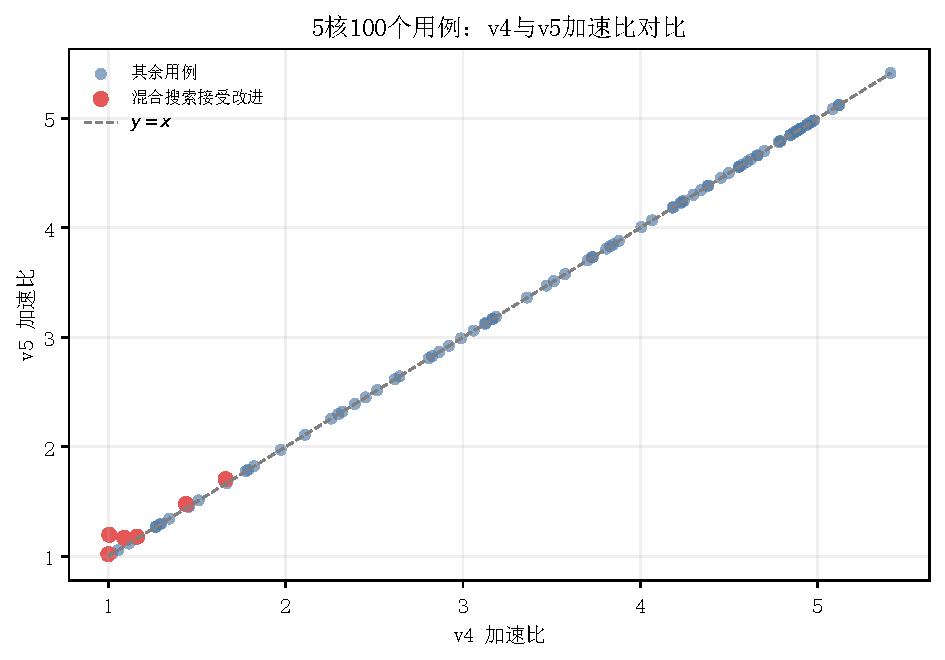
\includegraphics[width=0.78\textwidth]{figures/v4_v5_speedup.pdf}
\caption{100个用例的 v4 与 v5 加速比对比}
\label{fig:v4v5}
\end{figure}

\subsection{混合搜索接受的改进}

表~\ref{tab:accepted} 列出 20 个难例中最终被接受的 6 个方案。其他候选虽然完成了官方评估，但由于 Makespan 没有严格下降，均保留 v4 方案。

\begin{table}[htbp]
\centering
\caption{混合搜索接受的 Makespan 改进}
\label{tab:accepted}
\begin{tabular}{lrrrr}
\toprule
用例 & v4 Makespan & v5 Makespan & v5 加速比 & 规则 \\
\midrule
case\_009 & 92225 & 89919 & 1.704434 & hybrid\_id\_orig\_5 \\
case\_044 & 132892 & 131105 & 1.177735 & hybrid\_bytes\_load\_desc\_2 \\
case\_047 & 326508 & 320115 & 1.019971 & hybrid\_id\_orig\_2 \\
case\_066 & 249724 & 242906 & 1.478226 & hybrid\_id\_id\_7 \\
case\_069 & 25008 & 21040 & 1.195057 & hybrid\_id\_load\_desc\_5 \\
case\_071 & 17366 & 16183 & 1.169066 & hybrid\_id\_orig\_4 \\
\bottomrule
\end{tabular}
\end{table}

其中，case\_069 的 Makespan 从 25008 降至 21040，是本轮最明显的单例改进；case\_047 则从原先的单子图方案切换为 16 个连续 Task。由于问题一存在跨核等待和 DDR 竞争，增加分块数量并不必然带来收益，必须以官方事件模拟结果作为接受准则。

\subsection{合法性与可复现性检查}

最终方案的检查结果如下：
\begin{table}[htbp]
\centering
\caption{v5 方案的独立检查结果}
\label{tab:validation}
\begin{tabular}{lr}
\toprule
检查项 & 结果 \\
\midrule
用例数 & 100 \\
核心数 & 5 \\
方案结构校验错误 & 0 \\
官方问题一评估错误 & 0 \\
混合搜索候选用例数 & 20 \\
接受改进的用例数 & 6 \\
最小加速比 & 1.001797 \\
最大加速比 & 5.411518 \\
\bottomrule
\end{tabular}
\end{table}

所有数值均可由附件提供的 5 核 v5 汇总表和统计文件追溯；100 个最终方案均通过独立的结构检查。生成和合并命令为：
\begin{lstlisting}[language=bash,basicstyle=\scriptsize\ttfamily]
python code/hybrid_chain_search.py \\
  --worst 20 --official-budget 12 --population 16 \\
  --generations 6 --anneal-steps 40 \\
  --output day5_results/hybrid_search_delta.csv \\
  --plans-dir day5_results/hybrid_search_plans
python code/merge_hybrid_v5.py
\end{lstlisting}

\section{模型分析与问题一结论}

\subsection{方法有效性}

链簇规则的主要作用是同时减少切图边界和控制核心负载：连续规则保留长链局部性，负载加权规则降低 Pipe 最大负载，轮转和 wave 规则为宽浅图提供更多并行机会。混合搜索进一步在高层结构上改变组数、根链顺序和核心映射，避免直接随机移动单个 Op 导致子图环或大量无效候选。最终结果表明，混合搜索在 v4 的基础上仍能找到 6 个严格改进用例，但全局平均收益已经较小，说明剩余瓶颈主要来自官方仿真中的跨核等待、DDR 竞争和片上容量约束。

\subsection{局限性}

第一，搜索编码的是连续根组和核心映射，不能覆盖所有可能的非连续图划分，因此 v5 仍是启发式结果而非全局最优证明。第二，代理评分只用于预筛，不能替代官方模拟器；论文中的最终数字均来自官方评估结果。第三，算术平均对少数低加速比用例敏感，报告时应同时给出几何平均、中位数和总周期比，避免只挑选有利指标。

\subsection{结论}

问题一可以归结为带有 DAG、Task 顺序、核心映射和 DDR 搬运约束的离散调度问题。本文构造了“结构化候选生成—代理预筛—官方精确评估—混合局部搜索”的闭环。在 5 核、100 个用例上，最终 v5 方案的算术平均加速比为 $3.351113$，几何平均为 $2.982523$，总周期比为 $3.633128$，并且所有方案均通过合法性检查。该结果支持以下调度原则：深窄图优先保持连续链，宽浅图优先尝试负载均衡与轮转分组，最终方案必须以官方 Makespan 而非近似评分决定。
